\newpage

\section{Introduction}
\lhead{\textit{Introduction}}

It is the hope of the author that this document serves to persuade the reader of a number of things; firstly, persuasion can be thought of as an attempt to reason. Secondly, that reasons have a role in the likelihood of affecting cognitive change in the one who hears it. Finally, that different strategies for constructing reasonable arguments differ in their persuasiveness. 

It is apparent that persuasion occurs in the daily life of many, be it in advertisements, literature or dialogue, but, despite this, the definition must be clarified. In psychology, it can be defined as follows:

\begin{displayquote}
    Persuasion refers to any change in attitudes that results from exposure to a communication. ~\cite{Petty1986CommunicationChange}
\end{displayquote}


In order to model these changes in attitude quantitatively, one must understand something about them qualitatively first. Consider, for instance, a psychologist and their patient. Let the patient hold a set of beliefs that, to the psychologist, are subjectively incorrect, unhealthy or even dangerous. The role of the medical professional is to improve the health of their patient. As such, they will likely attempt to explain the perceived differences in their two opinions in order persuade the patient to alter the attitudes of the patient~\cite{Petty1997ThePsychology}. This view of persuasion as reasoning forms the basis of debate.

As such a prevalent phenomenon, it is well studied in psychology with a vast corpus of qualitative analysis that cannot be covered comprehensively in this document, therefore, only the most widely accepted model shall be discussed here, termed the Elaboration Likelihood Model (ELM)~\cite{Petty1997ThePsychology}. This framework was designed to provide a structure to the different methods and factors involved in the alteration of a set of sentiments. In psychophysiology, this can be seen as a change in valence or motivational intensity, aspects of an affective state~\cite{Harmon-Jones2013DoesScope}. It describes two ``routes'' to persuasion. The Peripheral Route describes influence that is achieved indirectly, through invoking a positive sentiment that an individual might associate with a notion or object. This method aims to alter a person attitude subconsciously. The Central Route is the more direct approach with arguments and reasons being exchanged without pretence. It is this Central Route that motivates the work that follows. 

In order to model influence via the Central Route, it is important to understand what variables impact it. For instance, the ELM describes a spectrum of the listener's predisposition to apply significant cognitive effort toward analysing an argument. Those who prefer to ponderously dissect a novel argument are most responsive to a strong argument, with few flaws, no matter who presents it. Alternatively, those indisposed to effortful thought surrounding an argument are much more likely to respond positively to the argument if it comes from a source they believe to be expert and reliable. Another impactful factor is the mood of the recipient of an argument, as those in a good mood are more likely to accept the argument, while those in a more negative frame of mind are more prone to counter-arguing. These factors combine in ways that the ELM does not have the precision to define mathematically, but nevertheless, aspects of the ELM shall be incorporated into the models described in \cref{sect:speaker_models} and \cref{sect:listener_models}.
 
 
One attempt at digitising the influence practised by human debaters, naturally, comes from Deep Learning. Some prominent technology companies, such as Google, Facebook and IBM, have involved themselves in pursuing Deep Learning as a method for devising communication techniques for both a communicator and an audience. \todo{Add more citations here.} For instance, there are those who seek to exploit the decision boundaries formed by a deep neural network by computing scene-independent perturbations to an input image that can effectively fool the network into misclassifying its target~\cite{Goodfellow2014ExplainingExamples, Brown2017AdversarialPatch}. This shows that, with adaptions to an input, the network can be persuaded to misclassify. An example can be seen in \cref{fig:adversarial_patch}. The fact that this perturbation can be independent of the context in which it is placed demonstrates a flaw in the performance of some neural networks for image-recognition. Here, the researchers exploit the network's desire to identify the most salient parts of an image and base its classification of the input heavily on that section. The patch shown here is designed to trick the network into believing that the patch is the most important region of the input image, and so the network bases its classification heavily on that region, disregarding what is intended as the input. This method of persuasion is powerful as it does not depend on the input or even, to some extent, the network it aims to fool as many of them are prone to this blinkered parsing of the input. 


\begin{figure}[H]
    \centering
    \includegraphics[trim={0, 7mm, 0, 0}, clip, width=0.7\textwidth]{Images/Misc/AdversarialPatches.png}
    \caption{An example of an adversarial patch applied to fool a deep neural network performing object recognition. The network can be seen correctly classifying the object contained within the image initially, but when the patch is introduced, the network instead focuses on the patch, incorrectly believing it to be highly relevant in the classification, and thereby ignoring the actual image intended for classification, in this case, a bannana. }
    \label{fig:adversarial_patch}
\end{figure}

Further work has been done in attempt to create agents capable of complex negotiation in natural language using deep neural networks. This report aimed to analyse a number of possible factors at play in successful negotiations, one of which is persuasion~\cite{Lewis2017DealDialogues}. Here, the authors attempt to train a pair of networks to negotiate a deal. They were each given an inventory of arbitrary objects and values and tasked with swapping them with another agent for a profit. They negotiated using a dataset of transcriptions of crowd-sourced interpersonal deal-making. This project failed to create agents proficient enough at using natural language to be successful, though, more troubling, they did learn to deceive their counterpart. This was due to the deceit practised by the humans that the networks were trained on and employed by the agents to attempt to get a better deal for themselves. A strategy they devised was to systematically understate their level of desire for their target product in an attempt to make the best possible deal. Similar behaviour can be observed in the field of experimental economics in~\cite{Smith1976ExperimentalTheory}, a seminal paper on market games. 

The pinnacle of persuasive deep learning methods comes from IBM, however. Project Debater is a project designed to provide a competitive debating engine that can, given a topic and a short amount of time, generate a compelling narrative in support of the claim it intends to make (see~\cite{Hou2017ArgumentModel, MassWordSpeech} for more detail). The agents goal is both to persuade the judges and respond to the opponent in a formal debate style. To achieve this, the agent is trained on a vast corpus of publicly available datasets, transcripts and Wikipedia articles. This requires the ability to identify which aspects of a sentence are most salient for the claim in question and therefore being able to draw out the information that may be most relevant, determine whether or not it is, and then finally incorporate it into a compelling speech~\cite{Levy2018TowardsSupervision}. The ``convincingness'' of the argument is learned from a manually labelled dataset created by people deciding the relative ``convincingness'' of one argument against another~\cite{Habernal2016WhichLSTM}. The authors determine that this is an effective tool in quantifying the power of an argument and the errors in the results are likely attributed to ambiguous topics rather than significant flaws in the design of the project. This project also aims to incorporate novel aspects of speech recognition into the agent's ability to comprehend its opponent's assertions and rebut them. Previous attempts at sentiment analysis in order to understand and analyse the content have been trained using text-based transcriptions of public debates. Project Debater includes the novel dimension of tonality by training on the auditory data to learn to identify the claim and sentiment of the speaker. The results of this work leave plenty of room for improvement but show that the field of listening comprehension can be incorporated into artificial argumentation and influence of opinion.

Much research has also been done in the area of opinion dynamics, as it is a useful tool to employ in swarm robotics. Understanding the evolution of ideas and motivations in a population is essential for creating rational behaviour in group. A broad description of rationality dictates that an agent must be autonomous, sociable, proactive and reactive~\cite{Genesereth1994SoftwareAgents, Castelfranchi1995GuaranteesArchitecture}. Under these tenets, the agents adhere to a set of rules to act in the best interests of themselves or the group without central oversight, working to produce a particular result more complex than any individual could produce alone~\cite{Rawls1971AJustice}. Consider the work of ~\cite{Parker2009CooperativeProblem}, in which the authors describe the need for a swarm of robotic agents to form a collective decision that is in the best interests of the population as a whole without reference to a central authority. This allows for a simple yet robust model as there is no central node in the network of communicating agents that, should it fail, would incapacitate the population. Inspiration for this was drawn from naturally occurring swarms of ant and bee colonies~\cite{Pratt2005BehavioralCurvispinosus, List2009IndependenceSwarms}. In this work, the agents are programmed with a set of simple rules allowing them to share and combine information amongst themselves, influencing each other into adopting a set of attitudes that best suits the needs of the colony. It suits the colony to collectively pursue one single desired outcome rather than dividing their resources in disparate pursuits of multiple unrelated goals. In short, it is better to work in concert toward a goal than in discord, even if the ultimate goal is sub-optimal, although optimality is usually preferred. This is only made possible through effective affective communication of opinions between the agents. 

The formulation of an individual agent's opinion can be mathematised via some ideas taken from uncertainty modelling, facilitating the analysis of their evolution~\cite{Wooldridge1995IntelligentPractice}. Assumptions can be made to facilitate modelling of abstract ideas such as opinions. This enables agents to reason on topics about which they are uncertain. One such assumption is the Closed World Assumption (CWA), which assumes that there exist a finite number of states that the agents' domain may be in~\cite{Jsang2001APROBABILITIES}. For illustrative purposes, consider a world containing $3$ possible states. This shall be demonstrated in two ways. Consider \cref{fig:hesse}. This diagram shows all the possible subsets of this $3$-dimensional world. The topmost set contains all the possible states of the world and so can be defined as $W = \{ H_1, H_2, H_3\}$. 

\begin{figure}[H]
    \centering
    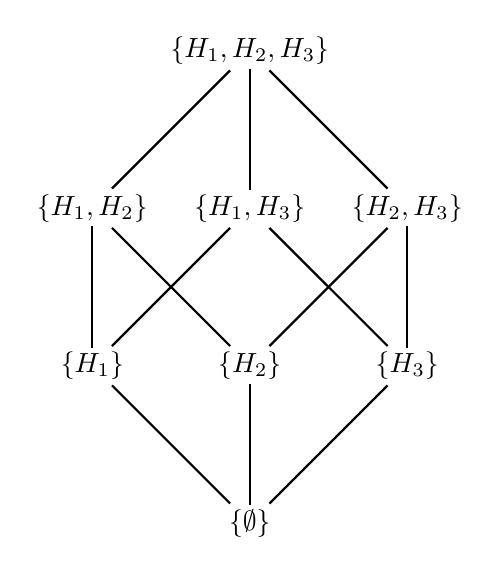
\begin{tikzpicture}
    % First, locate each of the nodes and name them
        \node (top) at (0,0) {$\{H_1, H_2, H_3\}$};
        \node (left) at (-2, -2) {$\{H_1, H_2\}$};
        \node (center) at (0, -2) {$\{H_1, H_3\}$};
        \node (right) at (2, -2) {$\{H_2, H_3\}$};
        \node (one) at (-2, -4) {$\{H_1\}$};
        \node (two) at (0, -4) {$\{H_2\}$};
        \node (three) at (2, -4) {$\{H_3\}$};
        \node (empty) at (0, -6) {$\{\emptyset \}$};

    % Now draw the lines:
        \draw [thick, shorten <=-2pt, shorten >=-2pt] (top) -- (left);
        \draw [thick, shorten <=-2pt, shorten >=-2pt] (top) -- (center);
        \draw [thick, shorten <=-2pt, shorten >=-2pt] (top) -- (right);
        \draw [thick, shorten <=-2pt, shorten >=-2pt] (left) -- (one);
        \draw [thick, shorten <=-2pt, shorten >=-2pt] (left) -- (two);
        \draw [thick, shorten <=-2pt, shorten >=-2pt] (center) -- (one);
        \draw [thick, shorten <=-2pt, shorten >=-2pt] (center) -- (three);
        \draw [thick, shorten <=-2pt, shorten >=-2pt] (right) -- (two);
        \draw [thick, shorten <=-2pt, shorten >=-2pt] (right) -- (three);
        \draw [thick, shorten <=-2pt, shorten >=-2pt] (one) -- (empty);
        \draw [thick, shorten <=-2pt, shorten >=-2pt] (two) -- (empty);
        \draw [thick, shorten <=-2pt, shorten >=-2pt] (three) -- (empty);
    \end{tikzpicture}   
    \caption{A Hasse Diagram for a world with 3 possible states.}
    \label{fig:hesse}
\end{figure}

This paradigm allows an agent to have a probability over each of the $n$ possible states in this world. This forms the basis of an agent's opinion, also referred to as a set of beliefs. These opinions can be combined with those of other agents in a variety of different ways. Thus, it becomes possible to assign a probability mass to each of the sets shown in \cref{fig:hesse} denoting the perceived likelihood of that set including the true state of the world. One of the axioms of this framework is that $P(W) = 1$, which intuitively makes sense as it must be the case that at least one of these states is true, although knowing this fact does not enlighten anyone who learns it. $P(\emptyset) = 0$ is equally informative. 

In published research, there are two prominent ways that agents share their full set of beliefs. The first involves each agent holding a set of beliefs over the state of the world, with a variable that alters the perceived reliability of each other agent individually, $\alpha_k$~\cite{Hegselmann2002Opinion}. At each moment in time, an agent $i$ averages together the opinions of all of its peers weighted by the reliability of each other agent in the population $\alpha_{k}, k \neq i$  to form its updated opinion $x(t+1)$. This seemingly simple model can produce some impressive dynamics, showing that just a few agents are key nodes in the social fabric of this population and that they have a disproportionate influence on the convergence of the system, though this is challenging to demonstrate analytically. Other similar models include~\cite{Deffuant2000MixingAgents}, \cite{Proskurnikov2017OpinionAgents} and~\cite{Friedkin1999SocialChange}. The Friedkin and Johnsen (FJ) model provides the closest analogue to the approach here taken, though different in that it is used to consider the effects of prejudice in the population. Importantly, the FJ model does include an element of an agent's past beliefs, which seems to be a logical inclusion. There is experimental evidence to suggesting there is some validity to the FJ model as it was tested on 50 groups of 4 students verifying that a more influential member of a population tended to emerge~\cite{Friedkin2011APower}. These experiments were constructed such that four students were in separate rooms faced with reaching a collective decision. They were able to make as many phone-calls to any other member of the group and had 20 minutes in which to make their decision. The emergent behaviour showed that generally a single member of the group quickly dominated the decision making process, revealing themselves as the most influential node in this artificial social network. 

A second approach is to consider the population with an outside perspective. In this model, a subset of the population is selected at random and ``pooled'' together, combining their opinions together at each timestep~\cite{Degroot1974ReachingConsensus, Lee2018CombiningConsensus}. This proposition allows for a variety of pooling operators that can affect the eventual collective decisions of the population. The methods proposed originally by DeGroot~\cite{Degroot1974ReachingConsensus} involve a linear combination of beliefs of the agents in a pool, though the models of Lee, Lawry and Winfield introduce nonlinear models that demonstrate aptitude at reaching a consensus under a variety of different possible circumstances. These pooling methods incorporate a generalisation of the idea ``two-heads-are-better-than-one'' as, in theory, the more individuals involved in the decision, the more information is likely to be available. In an anthropoid context, this phenomenon is also referred to as ``the wisdom of the crowd'' though there is some dispute as to its merits. It is assumed that $n$ individuals contain at least as much information as just one, but by the same token, the $n$ individuals contain at least as much misinformation~\cite{Dalkey1963AnExperts}. There is similar experimental evidence to support these pooling methods in a managerial technique referred to as the Delphi Method, despite being hardly oracular. Under this scheme, a panel of experts are gathered to reach a collective decision. They each answer a number of questions while isolated from one another. Then they are each presented with a summary of the responses from their peers and invited to update their own responses. This process is repeated until a predetermined condition is met~\cite{Dalkey1963AnExperts}. 

A common thread in the previous two methods is the combination of the agents full set of beliefs. Since this is not the method by which humans approach decisions, this report seeks to provide an insight into various methods by which only a subset or the most salient and persuasive information need be shared between agents in a simulated population~\cite{Harvey2019QuantitativeMarking}. With such an insight, it could become simpler to explain how a population of agents reach a certain decision, or persuade an agent with an erroneous set of beliefs too complex to change manually. This report aims to take a preliminary step in understanding aspects of the nuanced phenomenon of persuasion.

\Cref{sect:method} will outline the experimental set up for the models that will be described in \cref{sect:speaker_models}. The following section shall discuss the results found before suggesting a number of extensions to \cref{sect:speaker_models} that aim to more closely mimic anthropomorphic behaviours that incorporate aspects of persuasion. 


